% THIS IS SIGPROC-SP.TEX - VERSION 3.1
% WORKS WITH V3.2SP OF ACM_PROC_ARTICLE-SP.CLS
% APRIL 2009
%
% It is an example file showing how to use the 'acm_proc_article-sp.cls' V3.2SP
% LaTeX2e document class file for Conference Proceedings submissions.
% ----------------------------------------------------------------------------------------------------------------
% This .tex file (and associated .cls V3.2SP) *DOES NOT* produce:
%       1) The Permission Statement
%       2) The Conference (location) Info information
%       3) The Copyright Line with ACM data
%       4) Page numbering
% ---------------------------------------------------------------------------------------------------------------
% It is an example which *does* use the .bib file (from which the .bbl file
% is produced).
% REMEMBER HOWEVER: After having produced the .bbl file,
% and prior to final submission,
% you need to 'insert'  your .bbl file into your source .tex file so as to provide
% ONE 'self-contained' source file.
%
% Questions regarding SIGS should be sent to
% Adrienne Griscti ---> griscti@acm.org
%
% Questions/suggestions regarding the guidelines, .tex and .cls files, etc. to
% Gerald Murray ---> murray@hq.acm.org
%
% For tracking purposes - this is V3.1SP - APRIL 2009

% document format
\documentclass{acm_proc_article-sp}
%\documentclass[conference]{IEEEtran}

% set the path for graphics
%\usepackage{graphicx}
\graphicspath{{figures/png/} {figures/pdf/}}

% 0.85
\renewcommand{\baselinestretch}{1.0} 

\title{Continuous Transparent Authentication with User-Device Physical Unclonable Functions (UD-PUFs) based on Mobile Device Touchscreen Interactions}
%\subtitle{[Extended Abstract]
%\titlenote{A full version of this paper is available as
%\textit{Author's Guide to Preparing ACM SIG Proceedings Using
%\LaTeX$2_\epsilon$\ and BibTeX} at
%\texttt{www.acm.org/eaddress.htm}}}
%
% You need the command \numberofauthors to handle the 'placement
% and alignment' of the authors beneath the title.
%
% For aesthetic reasons, we recommend 'three authors at a time'
% i.e. three 'name/affiliation blocks' be placed beneath the title.
%
% NOTE: You are NOT restricted in how many 'rows' of
% "name/affiliations" may appear. We just ask that you restrict
% the number of 'columns' to three.
%
% Because of the available 'opening page real-estate'
% we ask you to refrain from putting more than six authors
% (two rows with three columns) beneath the article title.
% More than six makes the first-page appear very cluttered indeed.
%
% Use the \alignauthor commands to handle the names
% and affiliations for an 'aesthetic maximum' of six authors.
% Add names, affiliations, addresses for
% the seventh etc. author(s) as the argument for the
% \additionalauthors command.
% These 'additional authors' will be output/set for you
% without further effort on your part as the last section in
% the body of your article BEFORE References or any Appendices.

% acm
% \numberofauthors{3} 
% %  in this sample file, there are a *total*
% % of EIGHT authors. SIX appear on the 'first-page' (for formatting
% % reasons) and the remaining two appear in the \additionalauthors section.
% %
% \author{
% % 1st. author
% \alignauthor Timothy M. Dee\\
%       \affaddr{Electrical \& Computer Engineering}\\
%       \affaddr{Iowa State University}\\
%       \affaddr{Ames, IA, USA}\\
%       \email{timdee@iastate.edu}
% % 2nd. author
% \alignauthor Ian T. Richardson\\
%      \affaddr{Electrical \& Computer Engineering}\\
%      \affaddr{Iowa State University}\\
%      \affaddr{Ames, IA, USA}\\
%      \email{ian.t.rich@gmail.com}
% % 3nd. author
% \alignauthor Akhilesh Tyagi\\
%      \affaddr{Electrical \& Computer Engineering}\\
%      \affaddr{Iowa State University}\\
%       \affaddr{Ames, IA, USA}\\
%       \email{tyagi@iastate.edu}
% }

%IEEE
% \author{
% \IEEEauthorblockN{Michael Shell}
% \IEEEauthorblockA{School of Electrical and\\Computer Engineering\\
% Georgia Institute of Technology\\
% Atlanta, Georgia 30332--0250\\
% Email: http://www.michaelshell.org/contact.html}
% \and
% \IEEEauthorblockN{Homer Simpson}
% \IEEEauthorblockA{Twentieth Century Fox\\
% Springfield, USA\\
% Email: homer@thesimpsons.com}
% \and
% \IEEEauthorblockN{James Kirk\\ and Montgomery Scott}
% \IEEEauthorblockA{Starfleet Academy\\
% San Francisco, California 96678--2391\\
% Telephone: (800) 555--1212\\
% Fax: (888) 555--1212}
% }

\begin{document}

\maketitle
\begin{abstract}
%TODO remove the last sentence, mabe? Also, include numbers describing important results
A mobile device user continually interacts with many sensors through the natural
user interface (UI) of apps. 
These interactions are unique for each (user, device) pair
forming a user-device biometric.  
%
A physical unclonable function (PUF) can be realized
from the touch screen pressure variability.
%
We illustrate how a sequence of these pressure values 
from discrete touchscreen interactions 
may be used to uniquely characterize a user-device pair.
%
These touch screen interactions' Markov models can be integrated into a
continuous authentication layer.
%
Based on the most recent sequence of touch screen interactions,
the continuous authentication layer can assign a probability that these
interactions came from the authenticated (user, device) pair.
%
Continuous authentication helps protect access to a mobile device
from a malicious party by detecting the anomalies early.
%
Our experimental results show that this scheme can distinguish a user-device
pair from another with a confidence interval exceeding 70\%
with relatively few interactions. 
The false positive and false negative rates are below 12\%.
%
The execution time required for this authentication is 
on the order of a few hundred milliseconds, which suits mobile devices.
%
Increased data set sizes can push this accuracy into 90+\%.
\end{abstract}

% A category with the (minimum) three required fields
%\category{H.4}{Information Systems Applications}{Miscellaneous}
%A category including the fourth, optional field follows...
%\category{D.2.8}{Software Engineering}{Metrics}[complexity measures, performance measures]

%\terms{Theory}

%\keywords{physical unclonable function (PUF), user device physical unclonable function (UD-PUF)} % NOT required for Proceedings

\section{Introduction}
\label{sec:intro}
Mobile devices are increasingly becoming a repository of all our personal data and credentials.
This suggests increased attention to mobile device security.
The main gateway to any security schema is user authentication.
Biometrics based authentication schemes are less onerous and 
more transparent than the traditional password based authentication methods. 
Demonstrated in \cite{ScheelTyagi15}, a physical unclonable function (PUF) that composes human biometric with silicon biometric
leading to a unique user-device pair identity that is robust.
This PUF is based on the mobile device touch screen interactions.
The challenge is a polyline drawn on the screen. The user
traces this challenge line. The human pressure exerted in the trace and the exact traced path
profile captures the human biometrics of the user. This pressure is
processed through the capacitive touch
and sensor circuitry of the touch screen whose output captures the silicon biometrics, in a 
manner similar to the traditional PUFs. The touch events generated by the Android framework
contain pressure values which reflect both the human and the touch screen biometrics.
These pressure sequences can be quantized into binary responses
creating a challenge-response authentication framework. 
This PUF derives its randomness physically - from human behavior and silicon
transistor characteristics. 
The composition of the human and silicon components is not mathematically
modelable. This is what makes such an authentication framework robust. This polyline tracing authentication is relatively easy for a user - no passwords to remember
and it is fairly transparent.
 
Mobile device theft - particularly smartphones is a major problem. Consumer Reports \cite{CR14}
reported over 3.1 million smartphone thefts in 2013. Federal Communications Commission (FCC)
\cite{FCC14}
in its December 2014 report estimates 368.9 phone thefts per 100000 individuals in 2013. It states 
that about one third of crime involves a mobile phone. In NYC and San Francisco, the percentage
of crime involving mobile phones shoots up to 55-59\%. A mobile device has a time window right after
the theft wherein the unlocked authentication state still holds
which can be exploited by an adversary for considerable loss. 
This leads to the need for going beyond discrete time authentication - such as
password and touch screen PUF challenge response.

In this paper, we develop a continuous authentication framework based on touch screen based PUFs.
Touch screen interactions are an integral part of a mobile device UI. Many mobile apps use a soft keyboard. 
 If these user touch screen interactions can be captured to define a 
user model on a continuous basis, the user-device pair can be authenticated on a continuous
basis. The classical principles of spatial and temporal locality from computer architecture
are likely to hold in human behavior. Specific touch screen pressure token sequences representing
some phrases from email or messaging apps such as "I am OK" repeat over time giving rise
to temporal locality. Spatial locality weakly captures specific word sequences like "the" 
leading to pressure tokens of "t", "h", and "e". This locality comes from the language constructs for
English.

We modified a soft keyboard app to collect all the touch screen keyboard interactions data.
Android framework generates a sequence of MotionEvent objects in response to these touches.
The Android framework includes a class {\tt MotionEvent} (http://developer.android.com/reference/\\android/view/MotionEvent.html). 
The {\tt getPressure()}\\
method returns a normalized pressure value in the
range $[0,1]$ which is derived from the quantification of the current flow change due to
capacitive change. This pressure value
should reflect per device variability in the pressure measurement.
The continuous authentication layer (CAL) collects a sequence $S_{initial}$ of $N$ touch events' pressure
values $p_0, p_1, \dots , p_{N-1}$ from the user interaction within an app through the modified keyboard.
This sequence is processed for an $n$th order Markov model $M_{U, D}$ for the given user and device.
%Section \ref{} describes and example of a 2-Markov model to illustrate this concept.
Figure~\ref{fig:final_markov_model_state} shows an example of 2-Markov model.

% describes how the Markov model will look after it has been constructed
%TODO rephrase caption
\begin{figure}
\centering
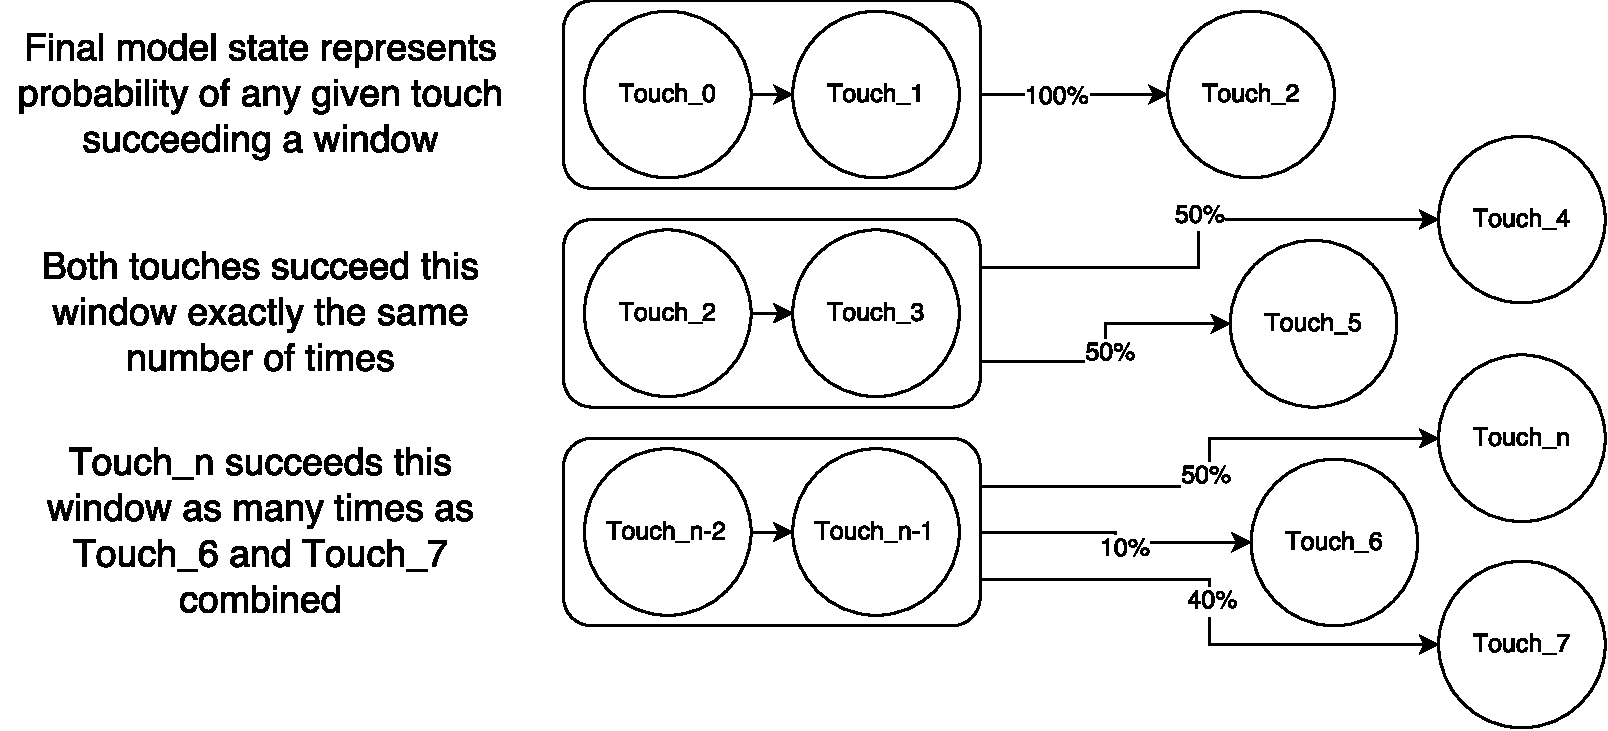
\includegraphics[width=.45\textwidth]{final_marcov_model_state.pdf}
\caption{
Example 2-Markov model after the probabilities have been calculated.
The rounded rectangles indicate 
a sequence of touch interactions 
which precede the following touch interaction with some probability $p$.
$p$ for token $T$ after sequence $W$ is computed 
as occurrences of $T$ after $W$
by occurrences of $W$.
% The top window states that 
% Touch\_2 succeeds the sequence Touch\_0, Touch\_1 with probability $100$\%.
}
\label{fig:final_markov_model_state}
\end{figure}

%describe in depth the continuous authentication scheme proposed, this is where the main contributions of this work should be discussed
The continuous authentication signature will fail if either the biometrically correct human user
or the biometrically correct device component is removed.
This paper builds a continuous authentication framework on user touch screen interactions.

Continuous authentication frameworks' basic premise is that a user behavior over time gravitates
towards  predictable. 
It can be frequently modeled as an $n$-Markov model. 
This model states that the user tokens of length $n$ repeat themselves with certain frequency. Hence if we can record history
of $n$-token sequences, they could help us classify the user's current behavior.
The tokens are touch screen pressure values that are continually generated
as the user interacts with an app through a soft keyboard.

In our system, we record touch pressures generated by 
users through the soft keyboard of an Android device. 
Once we have collected a sufficient number of touches, which is the training phase, we build 
a user profile or model.
%
This collection process can be transparent to the user,
happening in the background under normal use conditions. 
Future touch screen interactions are authenticated against this model.
%
Figure \ref{fig:authentication_accuracy} demonstrates that 
as few as $6000-8000$ touches may be used to achieve accuracies higher than $80$\%.
%
\cite{mackenzie1999text} reported that a
novice user can enter information through 
a soft keyboard at a rate of $20.2$ words per minute with
expert rates averaging $43$ words per minute.
%
A word consists of on average five letters, 
a rate of $101$ touch interactions per minute for the novice user.
%
This means in the average use case, a user can generate enough data to train
the model within $30-60$ minutes of soft keyboard use.
%
Hence the earliest this authentication can kick in
for a user-device pair is of the order of $30-60$ minutes.
%
This training can occur in a non-intrusive way
assuming the touch data is being collected over time in the background.

%TODO consider not saying this or at least revise it.
% describe the structure of the paper, what is contained in each section
The structure of the paper is as follows. Section \ref{sec:related_work} discusses related work. The $n$-Markov model and its parametrization are discussed in Section \ref{sec:modeling}. 
%Section \ref{touch_pressure_modeling} provides some implementation details with respect to how touchscreen pressure is used in the modeling scheme. 
Data collection methods are discussed in Section \ref{sec:data_collection}. The authentication scheme is presented in Section \ref{sec:differentiation}. The results including final numbers and 
their interpretation are given in Section \ref{sec:results}.
Section \ref{sec:PUF} discusses the variability and reproducibility properties of our system.
Conclusions are presented in Section \ref{sec:conclusions}. 

\section{Related Work}
\label{sec:related_work}

% show the range over which tokens are created
\begin{figure}
\centering
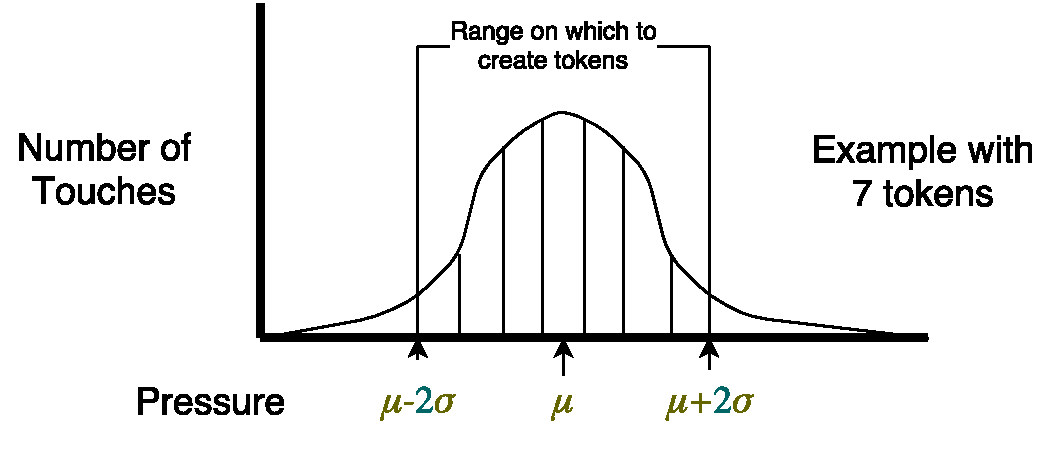
\includegraphics[width=.45\textwidth, keepaspectratio]{token_creation.pdf}
\caption{
Tokens are only created for 
pressure range $\mu \pm 2\sigma$ 
for each key.
Touches with pressure values
$p>\mu + 2\sigma$ and $p<\mu - 2\sigma$
are thrown out.
This eliminates outliers creating
increased reproducibility.
}
\label{fig:token_creation}
\end{figure}

% compare our work to other biometric work
There is significant amount of work on PUFs \cite{Devadas:2009:PUF}, \cite{PUFIntro}, \cite{Gassend:2002:SPR}
Ratha et al. \cite{Ratha:2001} proposed use of sensor biometrics for authentication.
%
In the continuous authentication world, a composite sensor vector \cite{zhu2013sensec} has been used to establish a user identity. 
This system, Sensec, builds the composite sensor
utilizing data from accelerometers, gyroscopes and magnetometers.
%
Other user biometrics such as inter key stroke timing 
\cite{KeystrokeHASE14},  accelerometer based signature \cite{Liu:2009:UAP}, MEMS sensors
\cite{Aysu:2013:DFL}, Gait sensors \cite{Gait}, gestures \cite{touchscreengestures}, \cite{Gesture14}, and 
broader sensor set \cite{Dey:2013:AHP} have also been
used. 
SenGuard \cite{shi2011senguard} is a similar to SenSec in creating a passive
authentication mechanism using sensor based models. In this paper, the continuous authentication is based on a combined user-device identity,
which is derived from a user-device (UD)-PUF \cite{ScheelTyagi15}.
%
\cite{ruhrmair2015virtual} presents the idea of
"virtual proofs of reality" 
also referred to as "virtual proofs" (VP).
The aim of this work on VPs is
to prove physical statements over digital communication channels.
%
Our work can be seen as
a VP of the user's presence at the touchscreen.

% citation mentioned in HOST review
Other works \cite{rosenfeld2010sensor} have proposed 
entangling physical measurements with sensor data
to produce PUFs.
%
The goal of \cite{rosenfeld2010sensor} is to 
extend the functionality of conventional PUFs
to provide authentication, unclonability, and verification of sensed values.
\cite{rosenfeld2010sensor} proposes the integration of PUFs into sensors
at the level of hardware.
These hardware PUF sensors use sensed values as part of the challenge,
generating a different response depending on the physical measurement.
%
The work in this paper uses software to exhibit
the capacity of standard touchscreen sensors to provide PUF functionality.

%TODO compare our work to other work which considers typing patterns

%describe a Markov model in general
%describe what it means to be an n-gram sliding Markov model
%describe in what way we a Markov model to describe a user, device pair (our Markov model of touch, pressure values.
%An n-gram sliding Markov model.
\section{Modeling a User-Device Pair}
\label{sec:modeling}
%describe the motivation for the use of a Markov chain
Raw touch interactions at a specific key in the soft keyboard square button
generates a raw pressure value in the range $[0,1]$. These pressure values are tokenized
into an input alphabet for the Markov model.

% describe what is a Markov chain
Markov Chains are useful in predicting and modeling systems whose behavior evolves through discrete states. 
The probability of transitions between states can be captured.
In general an $n$-Markov model states that the
user tokens of length $n$ repeat themselves with certain frequency.
Hence a user history of $n$-token sequences could help us classify the user's future behavior. The tokens are
% pressure, location (the key which is pressed)
%TODO potentially include pressure, location values
touch screen pressure values that are continually generated as the user interacts with an app
through a soft keyboard.

% Other information about Markov chains
% traditional use of Markov chains, text linguistic analysis
% Historically the Markov Chain has found applications in (statistics?)

% begin talking about the construction of the model
Instead of building a complete Markov model of the user behavior,
we build a collection of $n$-grams
which are frequently instantiated sequences of $n$ tokens.
We use $n$-sized sequences 
within a user interaction
generated token sequence as an
$n$-gram which approximates an $n$-Markov model.
$n$-grams were originally
used in natural language processing \cite{Brown:ngram}.

% shows the pressure density for one of our users
\begin{figure}
\centering
%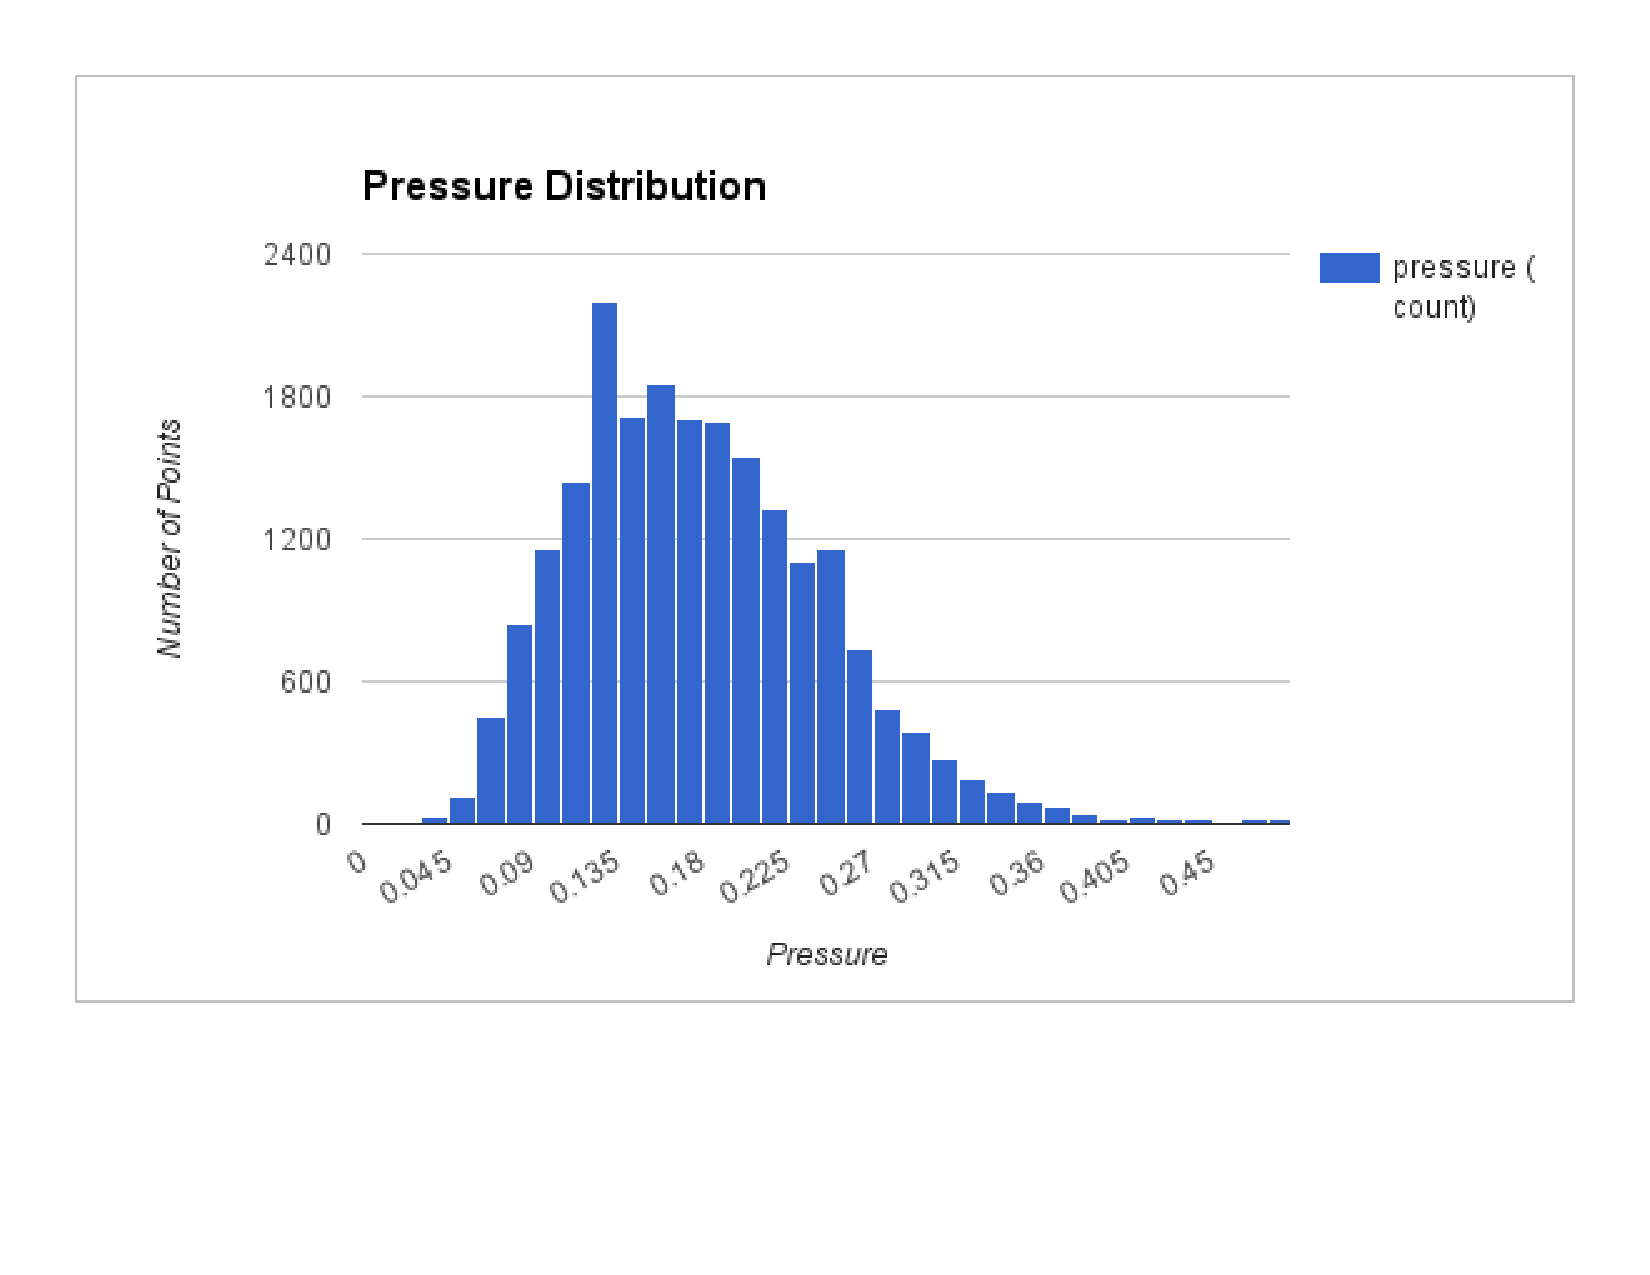
\includegraphics[width=.45\textwidth, keepaspectratio]{pressure_distribution.pdf}
\includegraphics[page=2, width=.45\textwidth, keepaspectratio]{Rplots.pdf}
\caption{
Density of touchscreen interactions' pressure values for one user.
%TODO say what is important about this observation
}
\label{fig:normal_distribution}
\end{figure}

% shows the qq-plot
\begin{figure}
\centering
%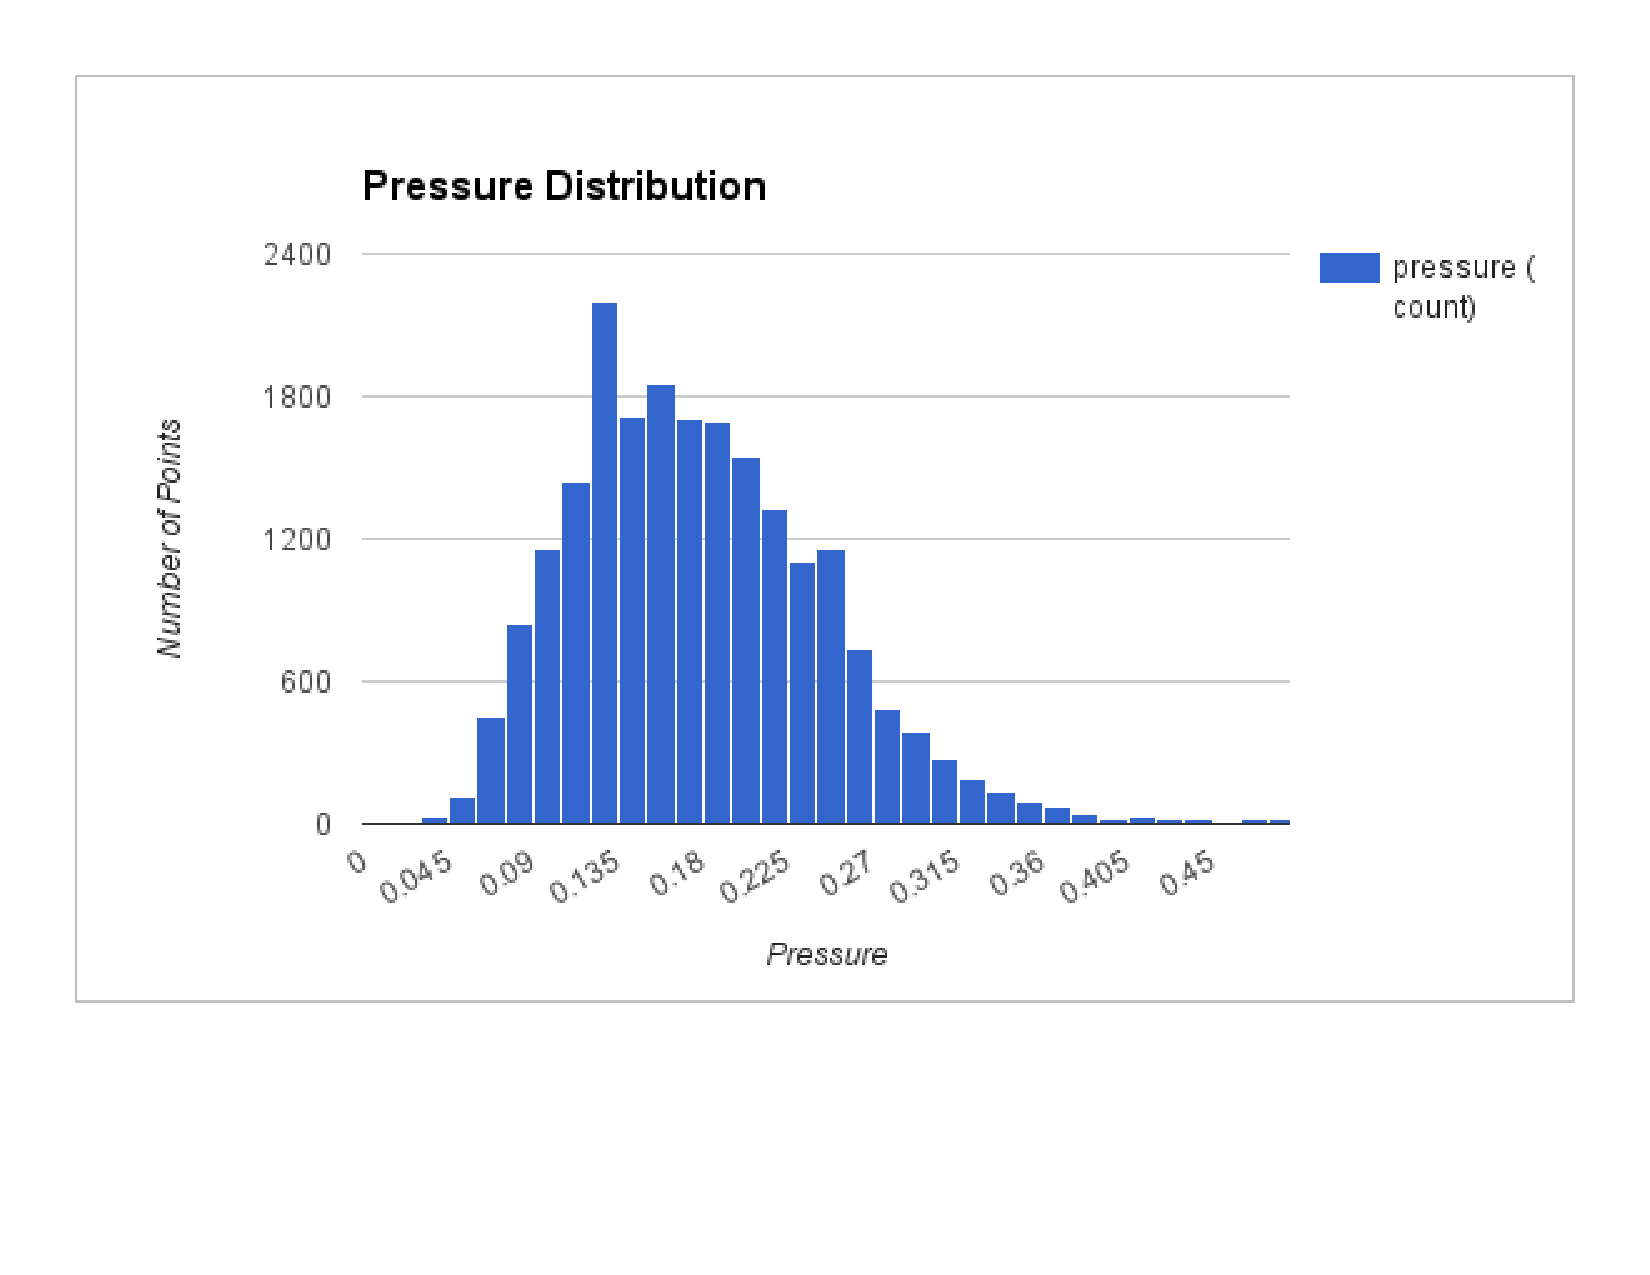
\includegraphics[width=.45\textwidth, keepaspectratio]{pressure_distribution.pdf}
\includegraphics[page=4, width=.45\textwidth, keepaspectratio]{Rplots.pdf}
\caption{
This Q-Q Plot describes data from
a data set having a right skew compared to normally distributed data.
}
\label{fig:qq_plot}
\end{figure}

%TODO continue talking about model construction.
%how are tokens constructed
%how are probabilities calculated
In building the model we remove some touches likely to be mistakes by the user or simply outliers in the data set.
The distribution of touch pressure values is calculated for each square button area on the touchscreen. 
In our system these areas correspond to keys of the soft keyboard.
In order to develop PUF reproducibility,
the distribution of touchscreen pressure needs to be examined.
%
The Shapiro-Wilk normality test\cite{shapiro1965analysis} was conducted
using $5000$ pressure points.
The results, {\tt W = 0.97244, p-value < 2.2e-16}.
$W=0.97244$ describes how closely the data conforms to a normal distribution.
$W=1.0$ would suggest the data set is perfectly normal.
$p-value=2.2e^{-16}$ indicates a low probability that
$W$ can be explained by chance variation.
%
The null hypothesis of the Shapiro-Wilk is
data comes from a normally distributed set.
$p-value<0.05$ suggests the null hypothesis should be rejected.
It is highly likely that the sample is not normally distributed.
%
The Q-Q Plot for this data, Figure \ref{fig:qq_plot},
suggests the distribution differs from normal
by a slight right skew.
%
Figure \ref{fig:normal_distribution} plots the density of 
touch pressures from one of the test users.
%
The Shapiro-Wilk normality test,
Q-Q Plot, 
and density plot
all suggest the touchscreen pressure data is not normally distributed.

% show that our data is normally distributed
% useful resource: 
%   http://mathforum.org/library/drmath/view/72065.html
%\textbf{
%To verify pressure values generated by user on a given touch screen user are normally distributed,
%we preform the following statistical hypothesis test.
%TODO prove that pressure values are normally distributed
%}

From the token sequence,
a normal distribution mean and variance ($\mu$ and $\sigma$) values are estimated for each soft keyboard key.
%
If a touch interaction's pressure value falls outside of
$\mu \pm 2\sigma$ for a given key, 
then the touch interaction is not included in any of the $n$-token sequences. 
Figure \ref{fig:token_creation} illustrates 
this tokenization process.
The pressure values falling within $\mu \pm 2\sigma$ are tokenized
into a predetermined number of tokens $k$. 
$k=7$ token ranges in Figure \ref{fig:token_creation}.
The value of $\mu \pm 2\sigma$ was chosen because statistically $95.45$\% of touches 
will fall withing this range for normally distributed data \cite{threesigmarule}.
%
Through the data is not normally distributed,
we can pick out values from which x.
$95.45$\% corresponds to $1.69$ theoretical quantiles in \ref{fig:qq_plot}.
The function of the Q-Q Plot is to 
compare two distributions.
By taking data $\mu \pm 2\sigma$,
equivalent to $0 \pm 1.69$ theoretical quantiles,
we capture user data which is
linearly related to a normal distribution.
In other words if the data in this range
were multiplied by some factor,
it would appear to have come from a normal distribution.
%
Tokens are compared both for the key (keyboard button) location and the tokenized pressure value.

% visually drive the process of token creation
% this shows a model with k=3
\begin{figure}
\centering
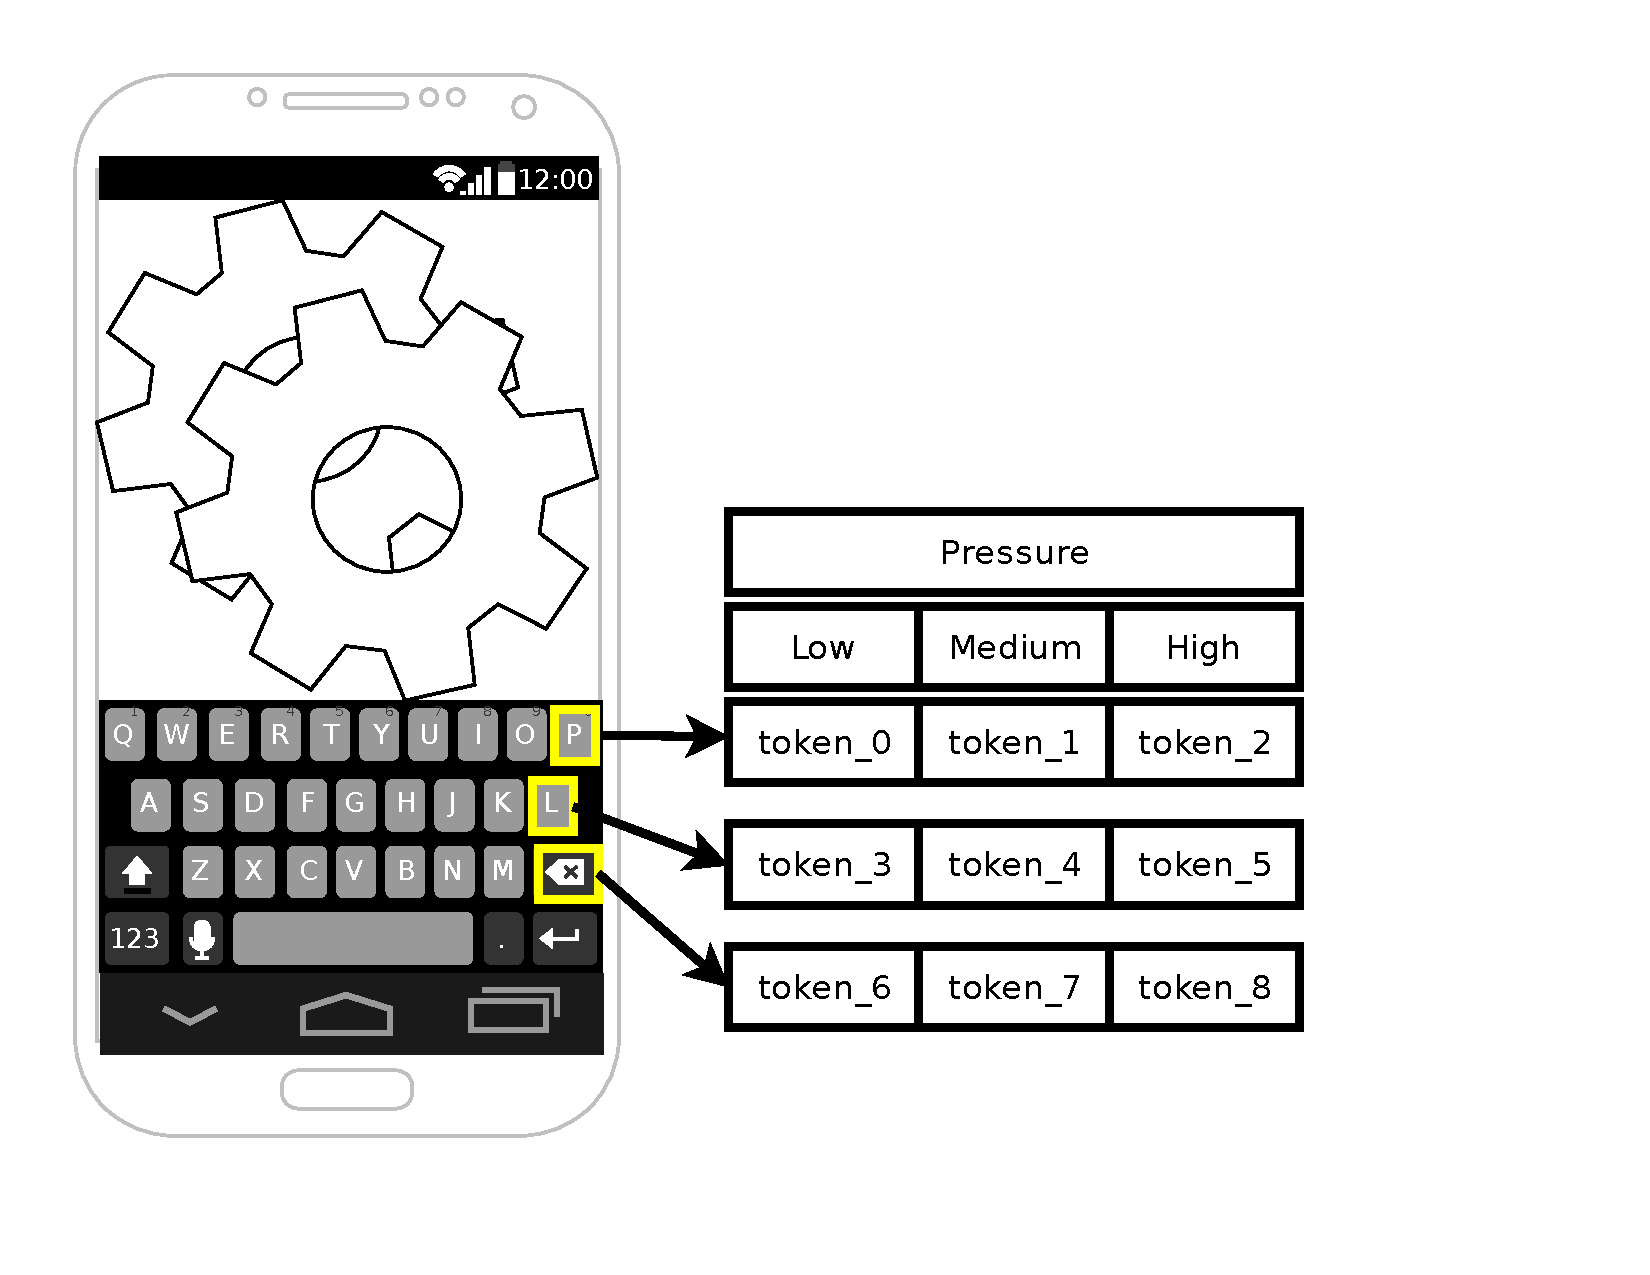
\includegraphics[width=.45\textwidth, keepaspectratio]{phone_tokens.pdf}
\caption{
Multiple tokens, $k=3$ above, correspond to each key location.
A touch screen interaction is assigned a token based on
key location and pressure.
}
\label{fig:phone_tokens}
\end{figure}

Figure \ref{fig:phone_tokens} demonstrates how
many unique tokens correspond to a single screen area.
In the example, the number of tokens per screen area is $k=3$.
This means that a user will create one of three unique tokens
when touching a given screen area.
Which token is created depends on the pressure 
the user applies to the screen area.
The total number of tokens used in the Markov model is equal
to the number of screen areas multiplied by $k$,
the number of tokens per screen area.

%TODO consider including this again
%n-gram a continuious sequence of n items
%markov model for comparason is built from a sliding model of the previous n touches
%describe how the Markov chain is applied to touch pressure to model a user
%this is a description of our specific implementation of a Markov model
%\section{Touch Pressure Modeling}
%\label{touch_pressure_modeling}
% this section should describe various implementation details

%TODO it may be useful to include all different parameters to the model, 
%TODO and the effects of varying each of them

% describe how the Markov model is built from the sequence of touch pressures
% describe the Markov model used
Our goal in modeling user touch screen interactions with a Markov model
is to classify the system in terms of its transitions between states. 
Each touch token contains information about the pressure and location 
of the interaction with the touchscreen.
These token fire off transitions.
In Figures \ref{fig:markov_model_building} and \ref{fig:final_markov_model_state}, 
Touch\_$n$ is a token and therefore comprised of a location and pressure range.
%
Given that the user can generate large number of possible pressure values,
ranges of pressure values are mapped to the same token as described above.
This is done in order to enable reproducibility.
This same approach works to help reduce the number unique locations.
Our implementation represents location based
on the key code associated with the key generating the interaction.
The effect of this is 
all coordinate pairs falling within the bounding box
of the key are mapped to the same token.
%
Tokens are considered distinct if
either the location or the pressure is different.
For instance, two user interactions with the same location
would be considered to be different tokens in the model if
the they fall within a different range of pressure values.
Additionally, two user interactions with different locations but with pressure
values within the same pressure range will be considered to be different touches.

%TODO redo this figure's caption
\begin{figure}
\centering
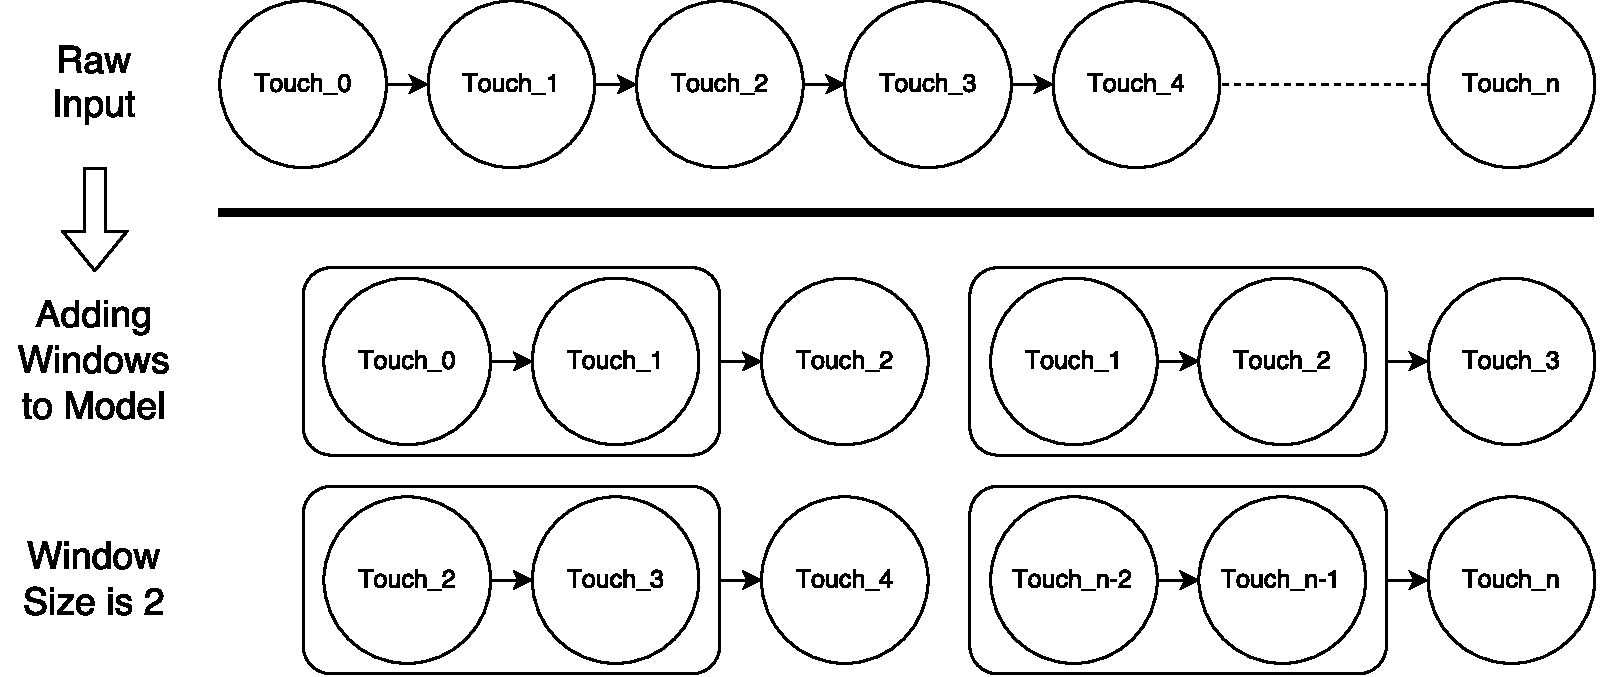
\includegraphics[width=.45\textwidth]{marcov_model_building.pdf}
\caption{
The top of this figure depicts the raw touchscreen interaction sequence.
Each touch represents a single interaction between the human user and the soft keyboard.
The diagram's lower portion demonstrates how the raw input is parsed into a 2-Markov model.
The bottom left image can be interpreted to say that Touch\_4 succeeds the sequence Touch\_2, Touch\_3 with some probability $p$.
}
\label{fig:markov_model_building}
\end{figure}

%describe how the model is constructed from the touch pressure sequence
Our Markov $n$-gram model calculates the probability of a given token following a specific 
token sequence of length $n$.
Given a training sequence of tokens $T_0, T_1, \dots , T_N$,
we use maximum likelihood estimation (MLE) as follows to build the model.
For all in-fixes of
length $n$: $T_i, T_{i+1}, \dots , T_{i+n-1}$,
the following $n$-gram model is created:
$P(T | T_{i..(i+n-1)}) =  count(T, T_i, T_{i+1}, \dots , T_{i+n-1})/\sum_{T \in \Sigma} count(
T, T_i, T_{i+1}, \dots , \\T_{i+n-1}))$, where $T_{i..j}$ represents the
token sequence \\
$T_i, T_{i+\\1}, \dots, T_j$.
Here, we are computing the probability of next token being $T$
given that the token sequence \\
$T_i, T_{i+1}, \dots , T_{i+n-1}$ has been seen.
It is just the
frequency of this event in the token sequence $T_0, T_1, \dots , T_N$. \\
$count(T, T_i, T_{i+1}, \dots , T_{i+n-1})$ is given by the number of in-fixes with the same value as
$T_i, T_{i+1}, \dots , T_{i+n-1}$ followed by the token $T$. This gives 
$count(T, T_i, T_{i+1}, \dots , T_{i+n-1}) = \sum_{j=0}^{N-n}(1$ if $T_{j..(j+n-1)} == T_{i..(i+n-1)} \&\&
T_{j+n} == T)$.

Larger $n$ increases accuracy of the true probability of a given token $T$ following
a sequence $T_{i..(i+n-1)}$.
The increased accuracy is due to the intuition that 
two users may behave identically for a sequence of $n$ tokens, but
differ in a sequence of $n+1$ tokens.
%TODO insert something here, doesn't flow
Figure~\ref{fig:markov_model_building} demonstrates how the token sequences for the Markov model are generated from the user's raw input from the soft keyboard.
%TODO describe this more

% describe the probability calculation in detail
Recall that the probability of a token $T$ following  a token sequence $T_{i..(i+n-1)}$ is 
expressed as the number of occurrences of $T$ succeeding the given sequence $T_{i..(i+n-1)}$ among
all the $N-n+1$ in-fixes of the sequence $T_{i..(i+n-1)}$.
The idea behind this probability calculation is illustrated in Figure \ref{fig:final_markov_model_state}.
Notably, Touch\_$n$ is not distinct.
In other words Touch\_$a$ will be considered equal to Touch\_$b$ if the keycodes of these touches are equal and the touches fall within the same pressure range. Pressure ranges are depicted in Figure \ref{fig:token_creation}.

%TODO talk about how prefix tree is used to store these sequences in order to increase the speed.
%TODO cite some source which supports the benefits of a prefix tree
%TODO explain what a prefix tree is
%TODO include some figures to illustrate what a prefix tree is
The algorithm to calculate the $n$-gram probabilities of
a token $T$ succeeding a given sequence
$T_{i..(i+n-1)}$ is the number of times that touch succeeds the sequence.
This counts the  number of 
occurrences of $T_{i..(i+n-1)}||T$,
where $||$ denotes concatenation.
The use of a prefix tree as a data structure helps keep track of appropriate
in-fixes and the affect of backtracking thus increasing the efficiency of this probability calculation.

% explain how the prefix tree is implemented in our system
In our system the $n$-token sequences are stored in a list
while a prefix tree is used to store pointers to the
instances of various tree prefixes in the list.
The prefix tree nodes also include the count of number of occurrences of a sequence.
This index list is useful because it eliminates the need to search the list in order to determine the successor tokens of
a given token sequence.
%TODO elaborate on prefix tree
%TODO explain why this increases the speed of the probability caluclation... articulate how an alternative data structure would perform

% gather touches over time
% eventually we have enough to authenticate
% authentication accuracy improves over time as more data is collected
Such a system might be incorporated 
into the Android environment in the following way.
A background service could be used to collect MotionEvent objects
from soft keyboard applications.
This would allow touch interactions to be collected over time.
A model of these touch events could then
be constructed in the background.
Periodic authentications could compare new touch interactions 
against existing older touches which have come from the user.
%
The number of touches used in the authentication could be
adjusted over time.
This would allow for lower accuracy models to be
constructed with relatively few touches while
higher accuracies would be achievable as
the system collects more touch interaction data.
The effect would be a small amount of added
security initially which improves over time.
%
Many things could be done if the result of this authentication
find the user is illegitimate.
One approach might be to lock the phone,
forcing the user to re-authenticate with some other method.

%basically the authentication scheme used
%frame it in more general terms, independent of our specific application
%\section{Differentiating \\A User-Device Pair}
\section{User-Device Pair Discrimination}
\label{sec:differentiation}
%TODO describe each of the model parameters in detail
%TODO state how each of the best model parameters were determined

%this figure describes how false positive and false negative percentages vary based on authentication threshold
\begin{figure}
\centering
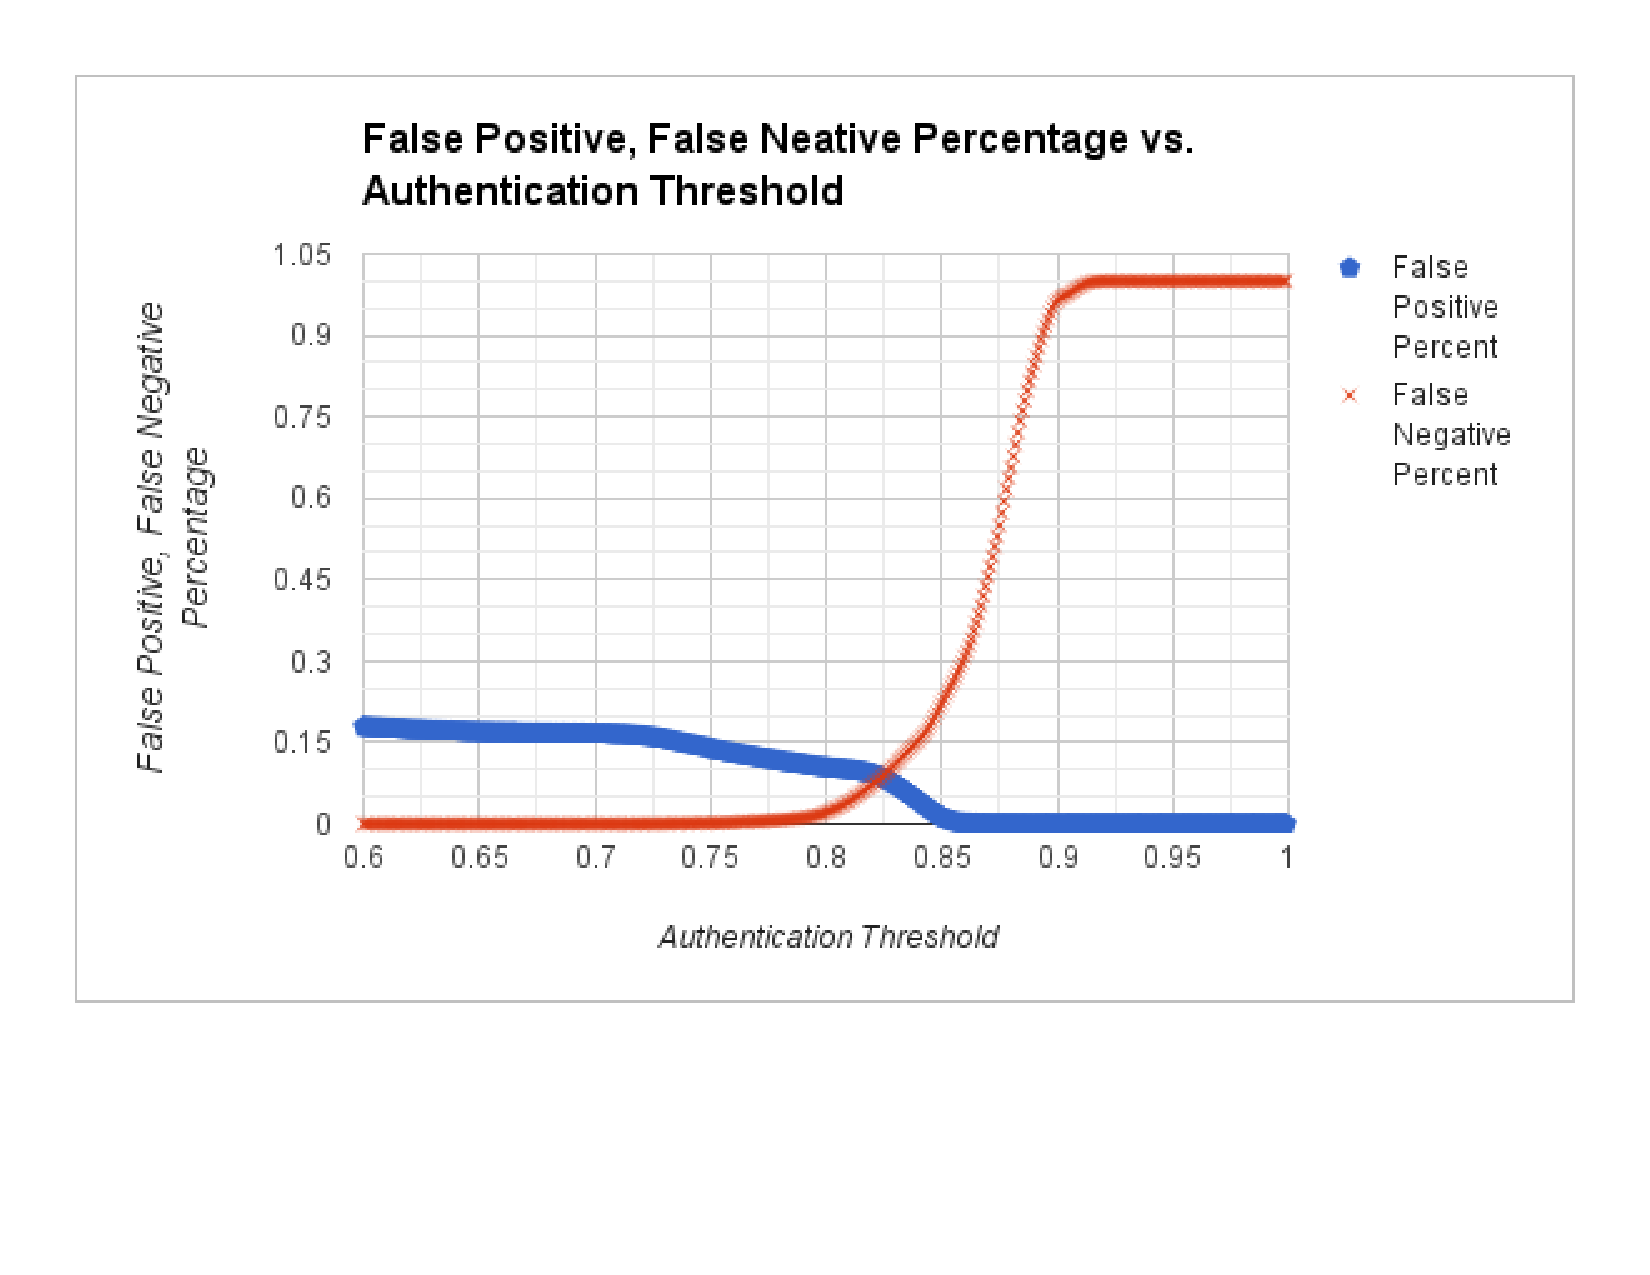
\includegraphics[width=.45\textwidth]{false_positive_vs_authentication_threshold.pdf}
\caption{False positive and false negative percentages vary as the authentication threshold is adjusted.}
\label{fig:threshold_vs_percentages}
\end{figure}

%TODO describe what the authentication threshold is
%TODO define false positive
%TODO define false negative
%TODO explain why the intersection of these two is significant in choosing the authentication threshold
In distinguishing one user from another user, 
the $n$-grams for the two users need to be compared. 
For a given $n$-gram 
$[(T_{i_0} T_{i_1} \dots T_{i_{n-1}}), (p_0, p_1, \dots, p_k)]$ where 
$(T_{i_0} T_{i_1} \dots T_{i_{n-1}})$ is the prefix sequence and 
$(p_0, p_1, \dots, p_k)$ is the
probability vector for the next token being 
Token $0$, Token $1$, $\dots$, Token $k$ from the alphabet $\Sigma$.
The distance between two $n$-grams 
$distance[(T_{i_0} T_{i_1} \dots T_{i_{n-1}}), (p_0, p_1, \dots, p_k)]$ and \\
$[(T_{i_0} T_{i_1} \dots T_{i_{n-1}}), (q_0, q_1, \dots, q_k)]$ is given by \\
$\Sigma_{j=0}^k|(p_j - q_j)|/(k+1)$ where $|x|$ is the absolute value of $x$.
The difference between two user profiles is 
the average difference between $n$-grams belonging
to the two profiles.
If the two $n$-grams are identical, the distance is 0.
One minus this distance is a measure of the {\it divergence} between two user profiles.

% what is the goal in preforming the above computation
Our continuous authentication system needs to determine 
when two sets of touch pressure values came from the same user-device pair. 
When authenticating a user, we take the difference between
the user profile $n$-grams constructed from the training data set 
and the $n$-grams constructed from the current touch interaction data.
The confidence interval that the current user is the same 
user who generated the training profile can be given by 
$1 - avgDistance(TrainingProfile \; n-grams, \; CurrentProfile \; n-grams)$. 
If the two profiles are identical with distance 0, 
confidence level in the user identity is highest at 1.
%
If authentication is a binary decision of yes or no, a threshold value $0 \leq th \leq 1$ is set.
if the ConfidenceInterval $= 1 -$ ProfileDistance $> th$, the user is authenticated; otherwise not. 

%TODO explain whether these distances are weighted or not
%TODO how are these distances weighted

%TODO authentication threshold described

% false positive, false negative percentage described
Figure \ref{fig:threshold_vs_percentages} illustrates how false positive percentage
and false negative percentage vary based on the threshold value for authentication.
These percentages are useful in quantifying the situations where
our implementation behaves incorrectly.
False positive percentage measures the fraction of positive authentications 
between two user-device profiles where 
the two profiles did not come from the same user-device pair.
False negative percentage is exactly the inverse of false positive percentage.
It describes the frequency with which the two user-device profiles 
from the same user-device pair fail authentication.

% significance of the intersection of false positive, false negative values
In Figure \ref{fig:threshold_vs_percentages} there exists a clear intersection between false negative and false positive percentages. This intersection is significant; at this point the system is not biased towards
either of false positive or false negative events. This point represents a balance in design. For our
data sets, this balance point was approximately at $th=0.83$. For a threshold in the range
$0.6 \leq th \leq 0.83$, false negative rate was close to 0 at the cost of a false positive rate approaching 0.2.
The choice of this threshold will depend on the authentication requirements.

% this figure describes the effect of window size on authentication accuracy
\begin{figure}
\centering
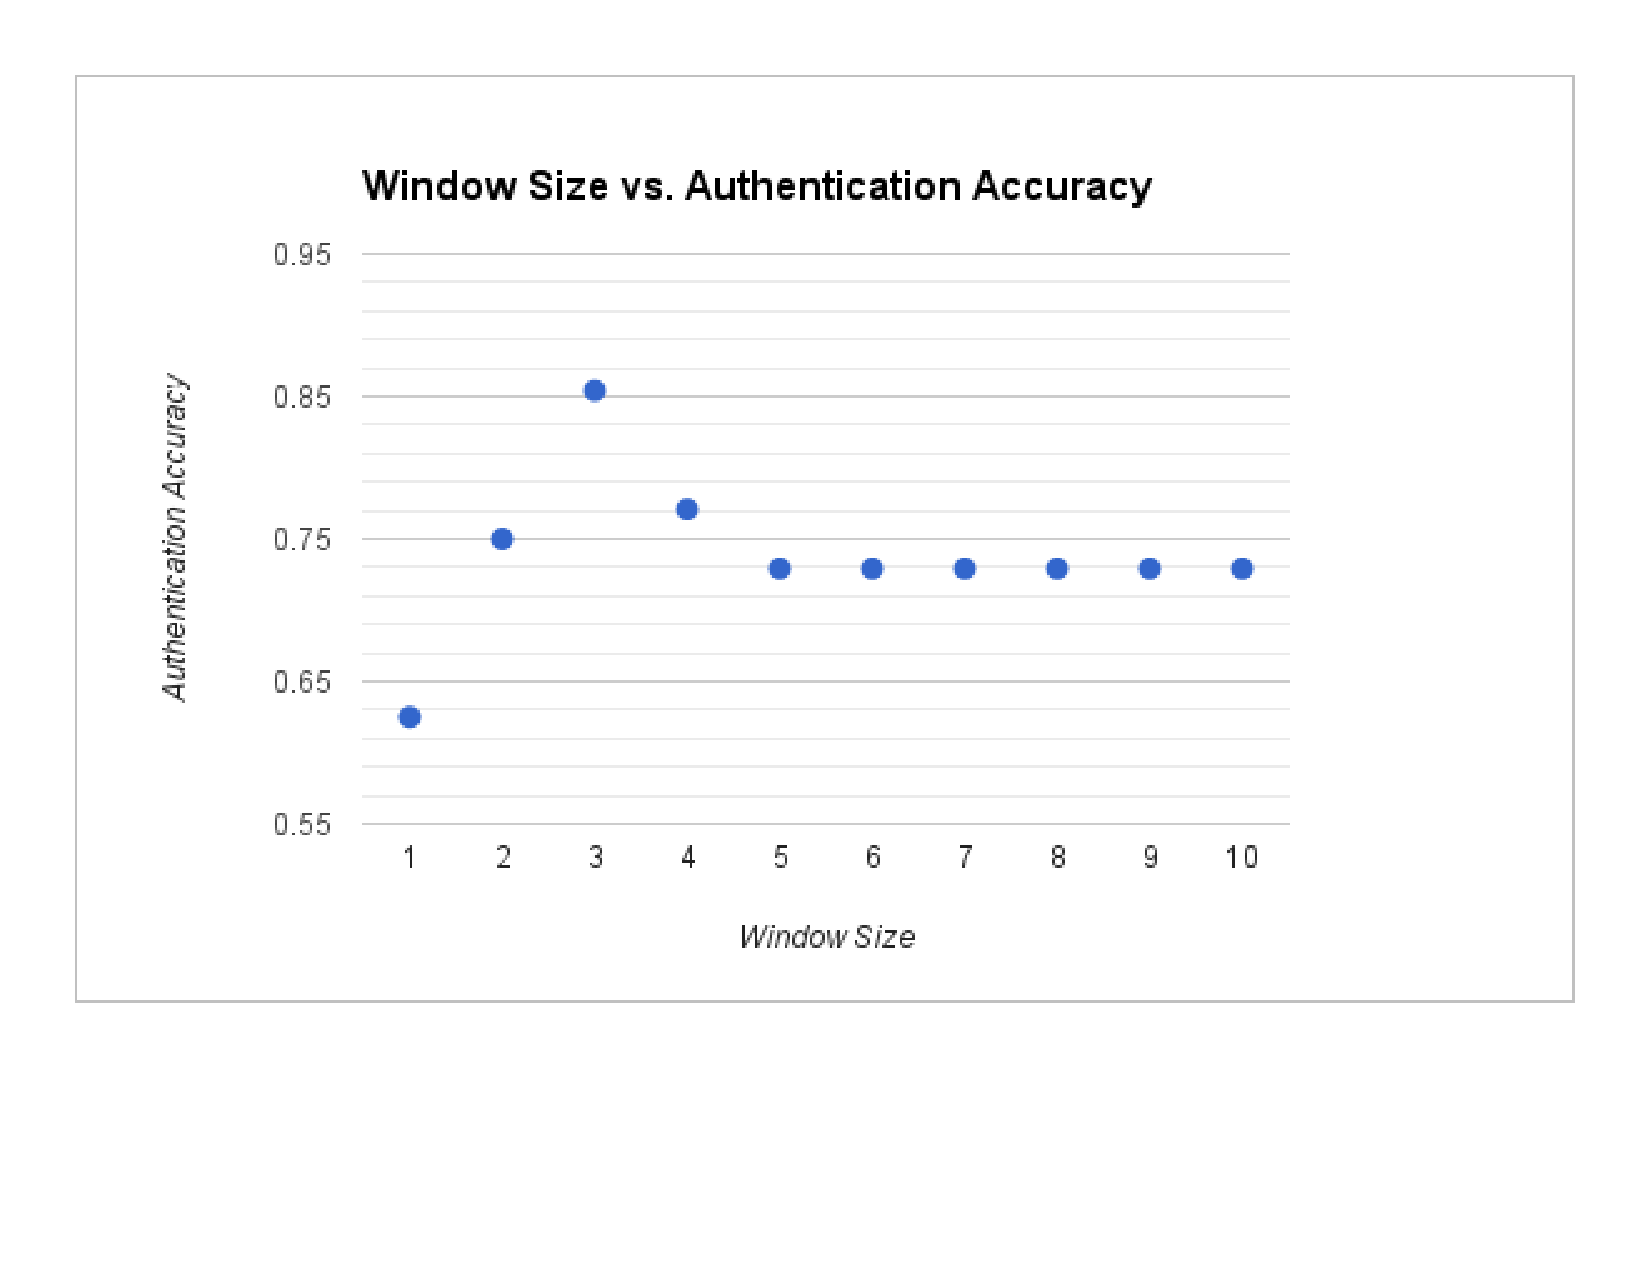
\includegraphics[width=.45\textwidth]{window_size_vs_authentication_accuracy.pdf}
\caption{The effect of $n$ in $n$-Markov Model window size on authentication accuracy.}
\label{fig:window_size_vs_authentication_accuracy}
\end{figure}

% describe the effect of window size on authentication accuracy
The link between model parameter window size and authentication accuracy is demonstrated by Figure \ref{fig:window_size_vs_authentication_accuracy}.
The window size parameter is equivalent to the $n$-gram size in our $n$-Markov Model.
The results in this chart were generated by 
holding all other model parameters constant and varying the window size. 
This approach was chosen to isolate the effects on 
authentication accuracy resulting from window size.
Window size achieves the greatest authentication accuracy at a size of $n=3$ with the authentication threshold set to $th=.75$.
Varying the authentication threshold to $th=0.9$, authentication accuracy reaches its maximum at $n=2$. 
The authentication threshold can be set at $th=0.5$ to achieve a result of $n=4$ providing maximum authentication accuracy.
From this we conclude that $n={2,3,4}$ to be viable options for this model parameter.

%TODO anything additional with regards to modifying statistics

\section{Data Collection and Analysis}
\label{sec:data_collection}
% describe the number of users from which the data was collected
% describe the method of collection
Touchscreen data for touch pressure models in this experiment 
was generated using a keyboard application created for the Android operating system. 
This keyboard extracts and records all necessary information 
from {\tt MotionEvent} objects generated by Android in response to
users' interactions with the keyboard.
This application was installed on Nexus 7 tablets.
Users were then asked to play a typing game 
in order to help expedite the data collection process.
After the users had generated at least ten thousand touches the data was collected from the user's device to train the profile.
%TODO put the data in context by detailing the number of touches collected from each user and the number of touches used to build the model
%
% describe the user base from which the data was collected for the results presented here
%TODO get data from more users
The results presented here are derived from the touch data generated by two users.
These users each used two different devices creating four user-device pairs
each having a large number of touch interactions.

On the Nexus 7 tablets,
the pressure data from the touchscreen is 
reported at a precision of $0.096$ by the {\tt getPressure()} method.
This measurement has been determined
by finding the minimum difference between
any two pressure values in one of our data sets.
%
There is a small probability the precision could
be greater if two adjacent pressure measurements
were never taken in the dataset.
%
The precision of {\tt getPressure()} is
known to vary among devices.
We have not encountered any inconsistency
in the precision among devices of the same type (eg. Nexus 7).

% describe how the data was analyzed
The collected data is analyzed using a program
developed to explore the effect of changing
parameters
$user\_model\_size$, $auth\_model\_size$,
$n$ window size, and $k$ token size
on\\
$authentication\_accuracy$.
%
The goal of the program is to
explore the space and determine which
set of a parameters maximize $authentication\_accuracy$.
%
The following section discusses the results 
produced by this program.

% what number of states exposed the most uniqueness e.g. how many tokens were best
% with what accuracy could users be distinguished from one-another
%
%TODO describe the performance of the system in terms of
% 1. aggregate performance
% 2. distinguishing user sets:
% 2.1. different user, different device
% 2.2. different user, same device
% 2.3. same user, different device
% 2.4. same user, same device
%
% this section describes how authentication accuracy was investigated. 
% Also included are a few figures which describe the best authentication accuracy percentage
\section{Results}
\label{sec:results}
%TODO discuss predictions and whether they were correct or incorrect.

% explain the contents of this figure.
% explain what each of the metrics used in the figure are.
Two key parameters are 
the training data set size,\\
{\it base\_model\_size}, and the 
authentication data set size,\\
{\it auth\_model\_size}.
Figure \ref{fig:authentication_accuracy} shows {\it authentication\_accuracy} 
as a function of {\it base\_model\_size} and {\it auth\_model\_size}.
We define {\it authentication\_accuracy} to be the percentage of authentications for which our system makes the correct decision.
That is $authentication\_accuracy = \frac{C}{T}$ where
$C$ is the number of correct authentications while
$T$ is the total number of authentications.
False positives and false negatives count against the {\it authentication\_accuracy}.
In other words, an authentic user is authenticated and a non-authentic user is not authenticated.
%
The size of base model and user model which result in a given authentication accuracy are aligned with that authentication accuracy on the horizontal axis in the chart.
The value of authentication\_accuracy can be read from the right y axis.
The model sizes can be read from the left y axis 
denoting the size in number of touches.
%
An example data point
might be read as follows: 
base\_model\_size of
6000 touches and auth\_model\_size of 6000 touches
results in 85\% authentication accuracy.

\begin{figure}
\centering
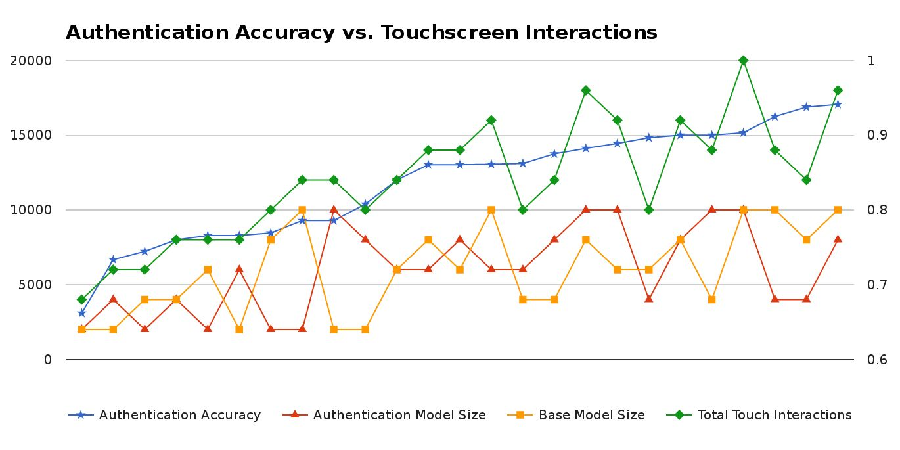
\includegraphics[width=.45\textwidth]{authentication_accuracy_vs_touchscreen_interactions.pdf}
\caption{
The left y axis describes the size of model
in number of touchscreen interactions.
We compare
authentication accuracy(blue star), measured on the right y axis, 
to authentication model size(red triangle),
base model size(yellow square),
and total touch interactions(green diamond)
measured on the left y axis.
Total touch interactions is the sum of
base model size and authentication model size.
}
\label{fig:authentication_accuracy}
\end{figure}

% explain why more touches does not always equal more accuracy
Both {\it base\_model\_size} and {\it auth\_model\_size} were varied between 2000-10,000 touches.
In some instances, 
increased numbers of touches did not result in higher\\
{\it authentication\_accuracy}.
% articulate the particular cases where this happened
% like when the base model is huge and auth model is small or something like this
An authentication model whose size exceeds the base model size by a significant margin usually
does not benefit the authentication accuracy.
%
A potential cause could be the distance computation 
between the base model (created from training) and the authentication model.
Existence of an $n$-gram in authentication model that does not belong to the base model
is considered an unlikely event, and hence an anomaly. 
This event is penalized in the distance computation
by computing absolute distance as its probability 
$Prob(NG[i, auth])$ - probability of an $n$-gram
$i$ in the base model.
Hence if this probability is $.75$, its contribution to
confidence interval is only $1-0.75=0.25$.
The authentication model includes some
$n$-gram sequences that were not seen in the training base model.
%
The difference between the $n$-grams is averaged
in order to generate the aggregate confidence interval.
Hence, $n$-grams which are found in the authentication model but not in the base model
decrease the aggregate confidence interval significantly.

% describes authentication accuracy dependence on the amount of user data
\begin{figure}
\centering
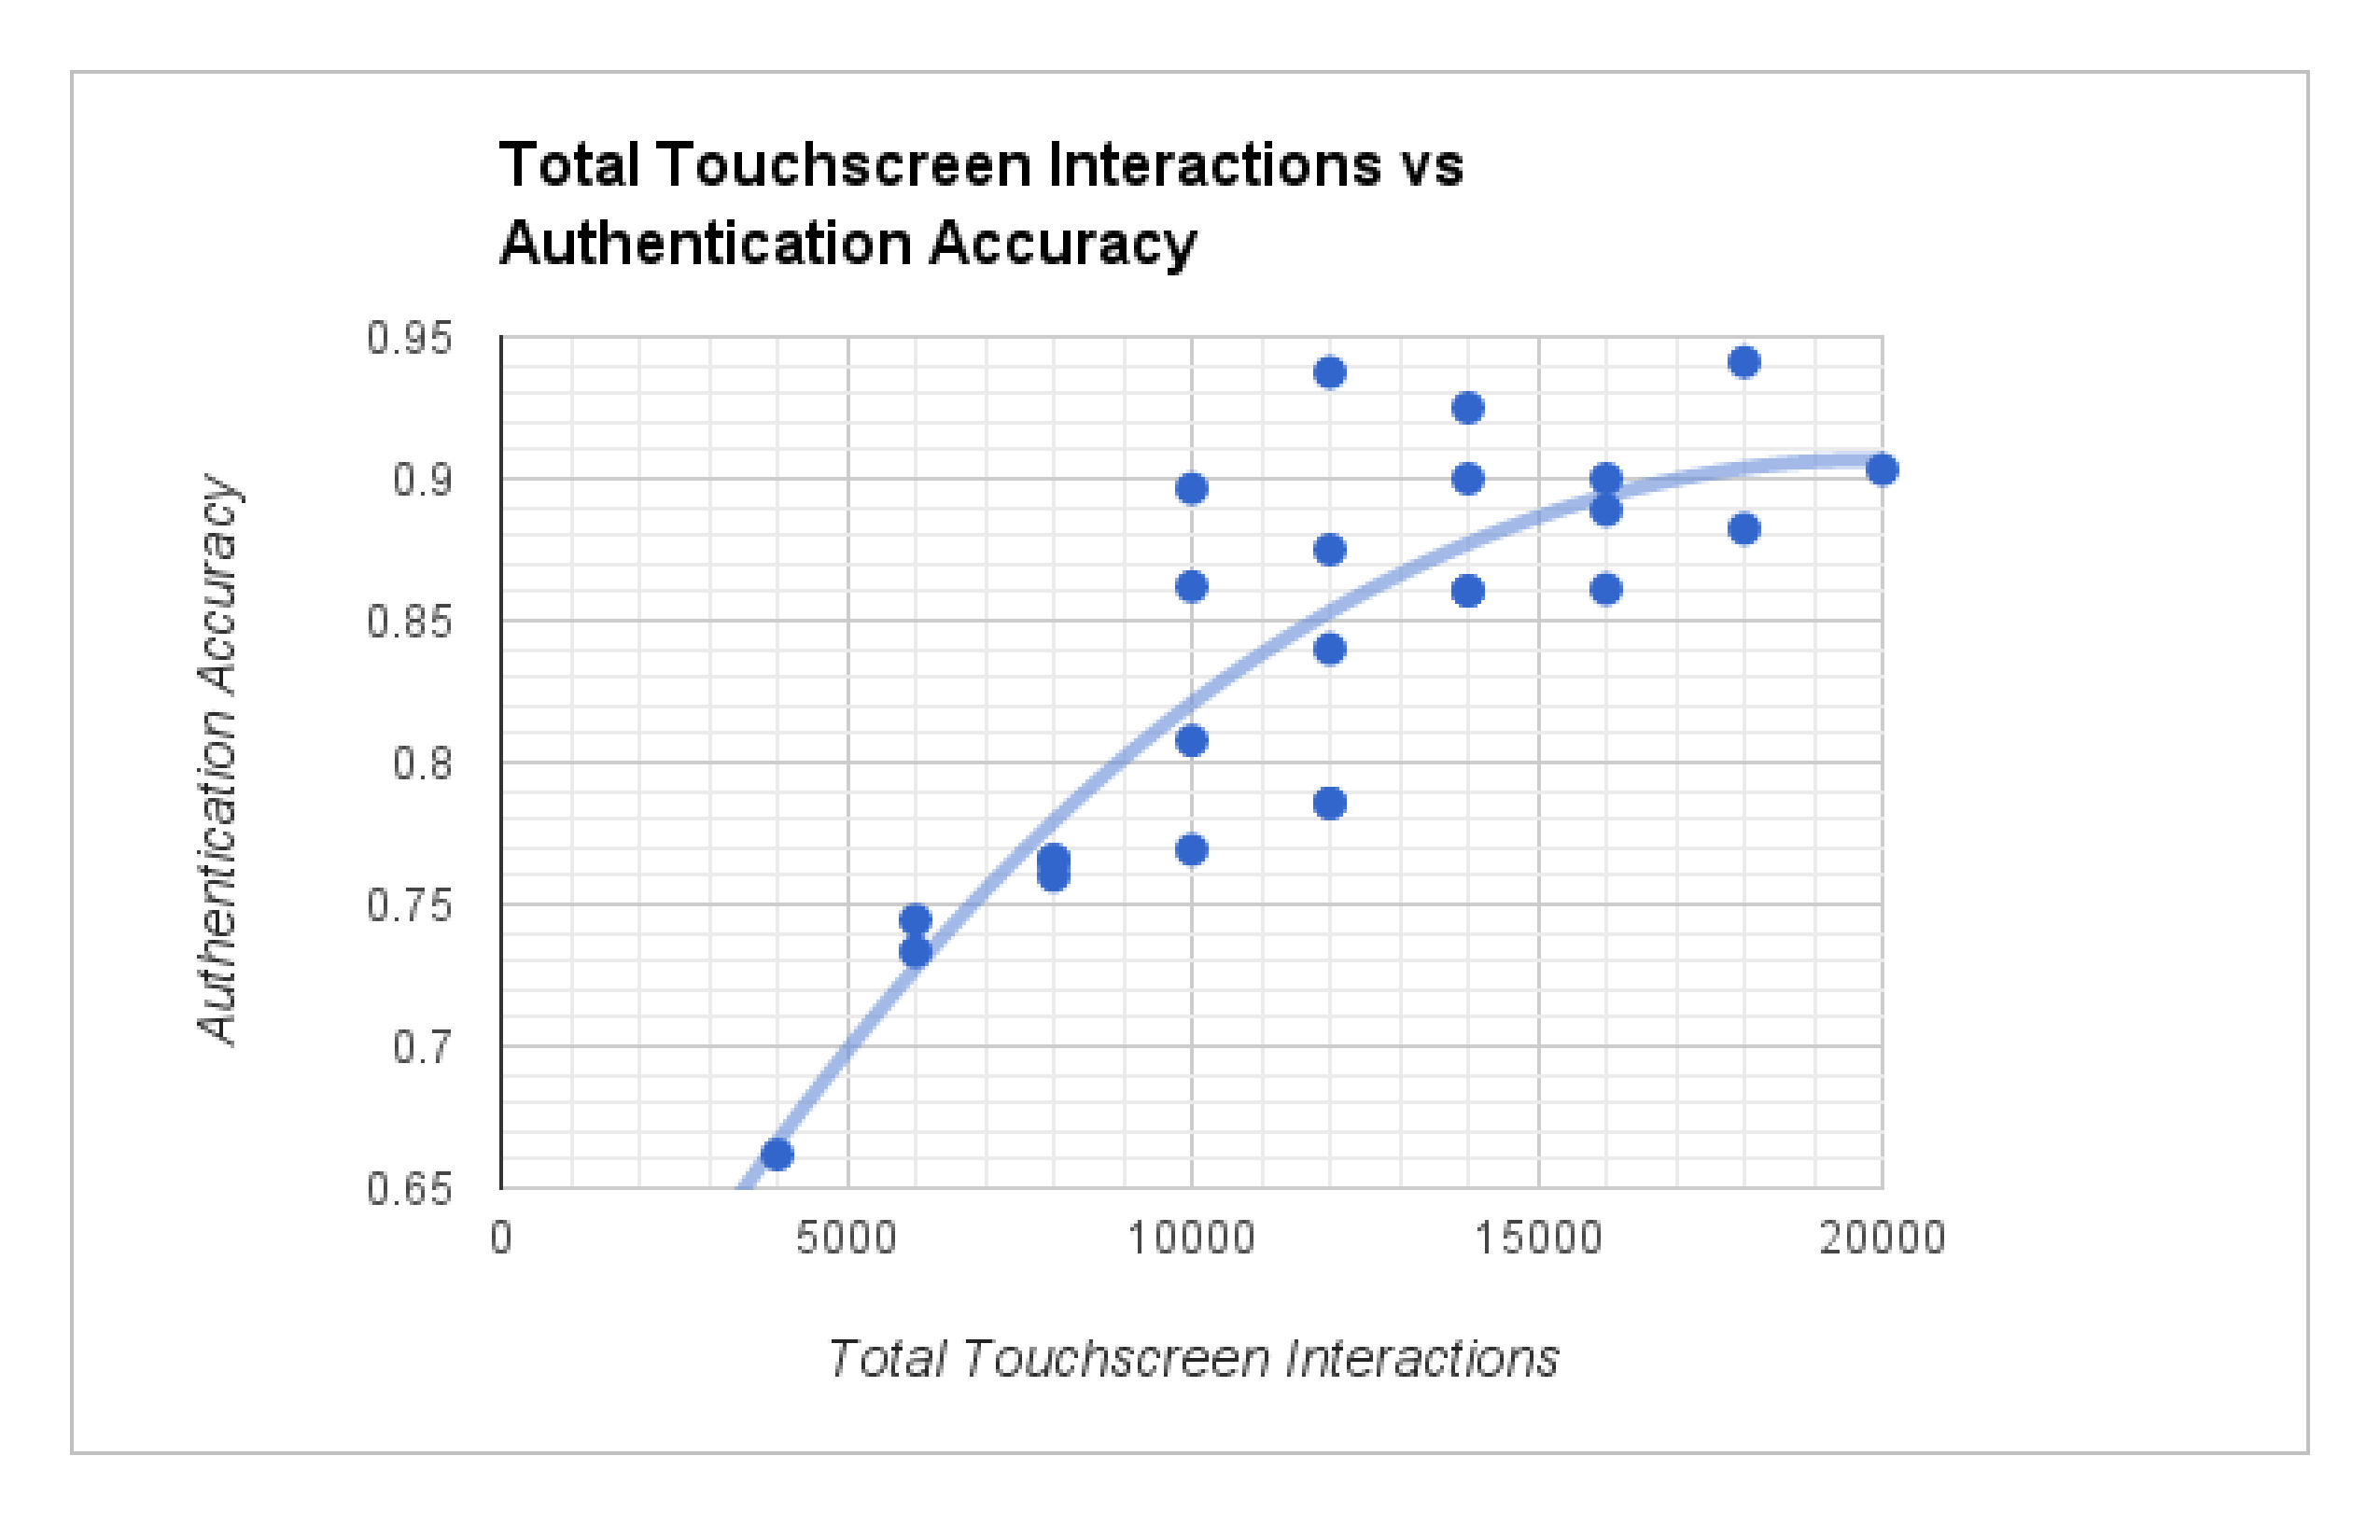
\includegraphics[width=.45\textwidth]{authentication_accuracy_vs_total_interactions.pdf}
\caption{
Authentication accuracy can be seen as
a function of
the total number of touch screen interactions
used in model construction.
Total touch interactions is the sum of
base model size and authentication model size.
}
\label{fig:total_touches_vs_authentication_accuracy}
\end{figure}

%TODO explain the contents of this figure.
% explain what each of the metrics used in the figure are.
Figure \ref{fig:total_touches_vs_authentication_accuracy} presents a trade off between the amount of data needed for an authentication and the accuracy of that authentication.
In general, more data will yield a better authentication accuracy, but this is not always true.
The size of the base model seems to contribute more to authentication accuracy then does the size of the authentication model, therefore, if the goal is to increase authentication accuracy it is better to increase the size of the base model compared to increasing the size of the authentication model.

% explain the contents of these figures.
% explain what each of the metrics used in the figure are.
Figure \ref{fig:nexus_total_size_time} displays
the execution time of our system on a Nexus 7 tablet.
Time taken is measured in milliseconds while 
total size indicates the total number of touch interactions used 
to construct both base and authentication models. 
%
The time metric does not include the overhead associated with adding touches to either the base or auth models. 
It is assumed this will be done over time as the user enters data.
In addition, adding touches is not a computationally intensive activity - more of a UI event. 
Time taken does capture 
the probability computation 
for base model and authentication model 
as well as the difference computation taken between the models.
%
In our current implementation,
we build the base model and authentication model in order to preform
the difference computation.
A potential increase in speed could be accomplished
by applying an incremental update to the models.
%
The effect is computation time required to preform an authentication is the sum of
base model construction time, 
auth model construction time, and
difference computation time.
This sum is what is depicted as computation time in \ref{fig:nexus_total_size_time}.
%
The benefit of the current design is increased ease of implementation, 
but this method suffers in execution time as a result.
%
The overall time taken is trending upward linearly in the total base model size and auth model size.
Time dependence on the number of touches is strongly related to
the probability computation.
An increase in the number of touches by $k$
increases the number of $n$-grams 
for which probabilities must be computed 
by $k$.

\begin{figure}
\centering
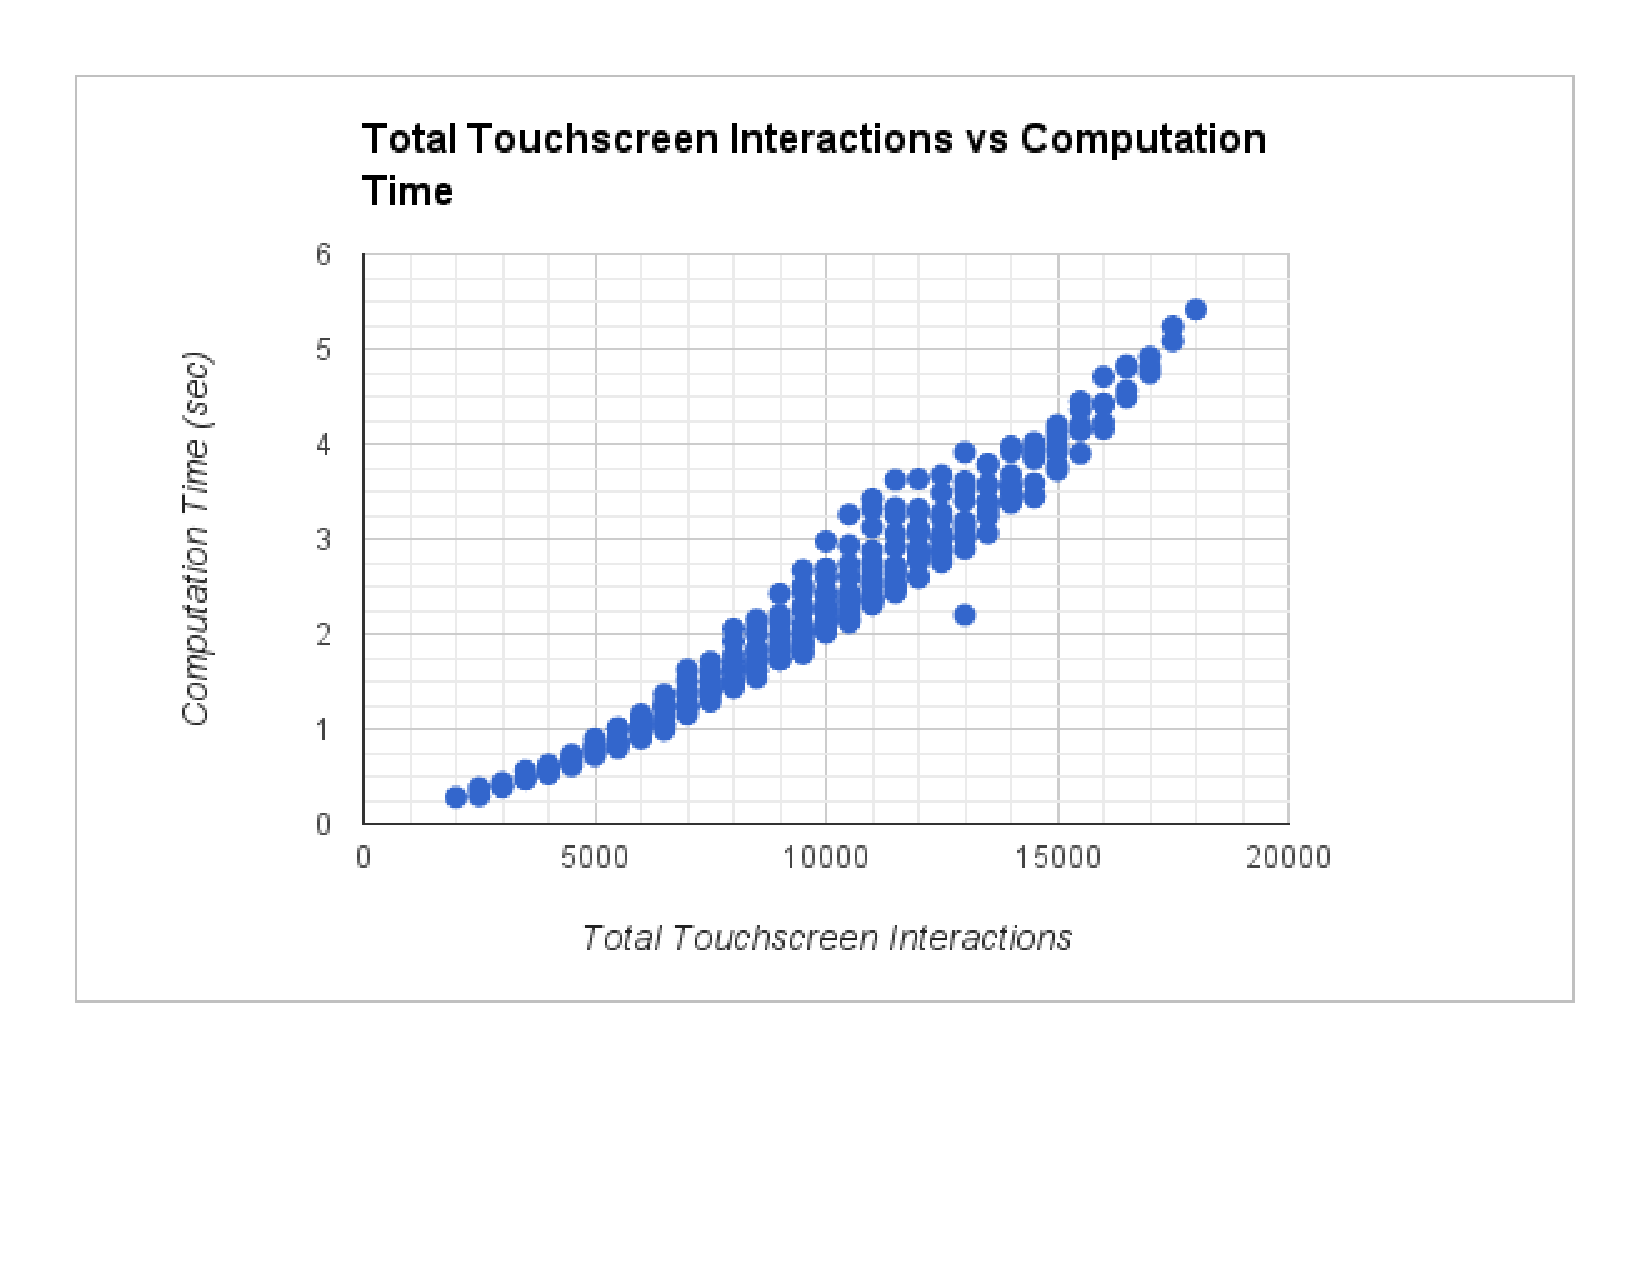
\includegraphics[width=.45\textwidth]{nexus_7_runtimes.pdf}
\caption{
The computation time, measured in seconds(sec), on a Nexus 7 tablet is
a function of
$Total Size =$ {\it base\_model\_size} $+$ {\it auth\_model\_size}.
Model sizes are measured by number of touch interactions used in their construction.
}
\label{fig:nexus_total_size_time}
\end{figure}

% point out that both authentication accuracy and time taken increase with Total Touches
%TODO this paragraph isn't very good or useful in it's current state, but the idea is good
Both {\it authentication\_accuracy} and time taken 
increase with total number of touches used in creating the models.
This observation suggests that the total number of touches
should be considered when targeting 
a specific computation time or {\it authentication\_accuracy}.
%
% Total touches, {\it authentication\_accuracy}, and time taken
% are related in the following way.
%TODO derive a mathematical function with the three
%
For a targeted accuracy, 
as Figure \ref{fig:total_touches_vs_authentication_accuracy} observes,
a certain minimum number of touches are needed.
This presents a problem if the execution time
resulting from this minimum bound on the
number of touches in the model is high. 
Our tests  on the Nexus 7 tablet show the execution time stays below 6 seconds
with the total number of touches in the model bounded by 18000.
Figure \ref{fig:nexus_total_size_time} shows this trade-off between number of touches
in the model and the corresponding execution time.

% tie it all together, discuss the importance of this section as a whole
Figures \ref{fig:authentication_accuracy}  \& \ref{fig:total_touches_vs_authentication_accuracy}
establish that in general a greater number of touches used 
in the authentication will result in a greater accuracy. 
This trend manifests in the charts as the peaks of highest authentication accuracy  
corresponding to the largest numbers of touches. 
Figures \ref{fig:nexus_speed_test} and \ref{fig:nexus_total_size_time} 
demonstrate the performance trade off associated with increased numbers of touches. 
As expected, increased authentication accuracy 
comes at the expense of execution time and more touchscreen data.

% (UD-)
\section{Distributed User-Device PUF}
\label{sec:PUF}
The preceding discussion extends the human-device entangled PUFs \cite{ScheelTyagi15} to a distributed implementation. 
The $n$-Markov model also determines frequently occurring $n$-token sequences for a
given user.
All of these $n$-token sequences can be considered to be the challenge set.
The resulting pressure value responses 
can then be quantized into a binary response in the same way as in 
\cite{ScheelTyagi15} resulting in the same variability and reproducibility properties. The main 
difference is that this distributed PUF is derived 
as a side-effect of the authentication mechanism.
This could support alternate functionalities that can benefit from a PUF based on the user-device physical randomness.

\section{Conclusions}
\label{sec:conclusions}
%TODO make sure to re-tell the story in the conclusion.
%TODO describe what has been presented in the paper
This paper presents a continuous authentication approach for mobile authentication.
We demonstrate that a sequence of pressure values generated through
discrete touchscreen interactions can be used to 
uniquely characterize a user-device pair.
%
These values depend on the physical properties
of both the user and the device 
giving rise to a user-device biometric.
%
A continuous authentication model prevents data theft 
from a mobile device even for lost devices.

%TODO describe how this might be integrated into the android environment
% number of touches collected over time
% continue building model in the background
% occasionally authenticate the newest sequence of touches against older training data

%TODO describe the implementation, model, authentication

%TODO discuss the advantages to using an n-Markov model over other modeling systsms

%TODO possible, describe applications  in terms of continuous authentication

Our experiments establish optimal 
training data set sizes around 6000-10000 touches, 
an authentication data set size at around 4000 touches, and 
the $n$-gram sequence length in the range 2-4. This leads to
authentication accuracy over 80\% with both false positive and 
false negative rates contained below 12\%.

\bibliographystyle{unsrt}
%\bibliographystyle{acm}
\bibliography{bibliography/markov_chains,bibliography/pufs,bibliography/other,pufs}

\end{document}
